\section{INITIAL SHEAR MODULUS AND N-VALUE 初始剪切模量和N值}

\begin{paracol}{2}
    
    The well-shooting test is gradually being adopted widely , because it is proven to be provided with such advantageous features that : 
    \begin{enumerate}
        \item eimmate any necessity o securing an extensive area for measurement;
        \item ensure higher accuracy of measurement, compared with surface refraction method;
        \item allow wave velocity measurement in a soft soil layer, even if there exists a hard layer above it.
    \end{enumerate}

    \switchcolumn

    地震测井试验试验正逐渐被广泛采用,因为事实证明它具有以下优点:
    \begin{enumerate}
        \item 消除了任何必要,确保了广阔的测量范围;
        \item 与表面折射法相比,确保更高的测量精度;
        \item 即使在软土层之上,也可以进行波速测量。
    \end{enumerate}

    \switchcolumn*

    A review of the data on the well-shooting tests conducted in the past has led the authors to take notice that there have been a number of instances where the well-shooting test and the standard penetration test were conducted on the same site. It is therefore necessary to make an investigation into the relationship between the shear modulus and the N-value of soil deposits obtained respectively by the well-shooting test and the standard penetration test, so as to get a better knowledge of elastic properties of soil. When the value of initial shear modulus and N-value are to be sampled from the existing data, it is necessary, however, to set up certain criteria to avoid any partial data sampling.

    \switchcolumn

    对过去进行的地震测井试验数据的回顾使作者注意到,在许多情况下,在同一地点进行了地震测井试验和标准贯入试验。 因此,有必要对分别通过地震测井试验和标准贯入试验获得的土壤沉积物的剪切模量与N值之间的关系进行研究,以便更好地了解土壤的弹性。 但是,当要从现有数据中采样初始剪切模量和N值时,有必要设置某些标准以避免任何部分数据采样。

\end{paracol}

\Paragraph{Criteria of Data Sampling 数据采样标准}

\begin{paracol}{2}

    In the case of the authors' investigation, criteria of data sampling were set up so that such data as might meet the following requirements could only be adopted :

    \switchcolumn

    在作者调查的情况下,建立数据采样标准,以便只能采用可能满足以下要求的数据:

    \switchcolumn*

    \begin{enumerate}
        \item Soil has to fall under the category of cohesive soil.
        \item Shear wave velocity has to be measured by way of the well-shooting test.
        \item Uniform section of shear wave velocity values and N-values has to be more than 2.0 m, as shown in \autoref{figure:10} "An Example of Data Sampling."
        \item The well-shooting test and the standard penetration test have to be conducted on the same site.
    \end{enumerate}

    \switchcolumn
    \begin{enumerate}
        \item 土体必须属于黏性土体。
        \item 剪切波速度必须通过地震测井试验来测量。
        \item 剪切波速度值和N值的均匀截面必须大于2.0 m,如\cnfigureref{figure:10}“数据采样示例”所示。
        \item 地震测井试验和标准贯入试验必须在同一地点进行。
    \end{enumerate}
    
\end{paracol}

\begin{figure*}[!htb]
    \begin{minipage}[t]{0.50\textwidth}
        \centering
        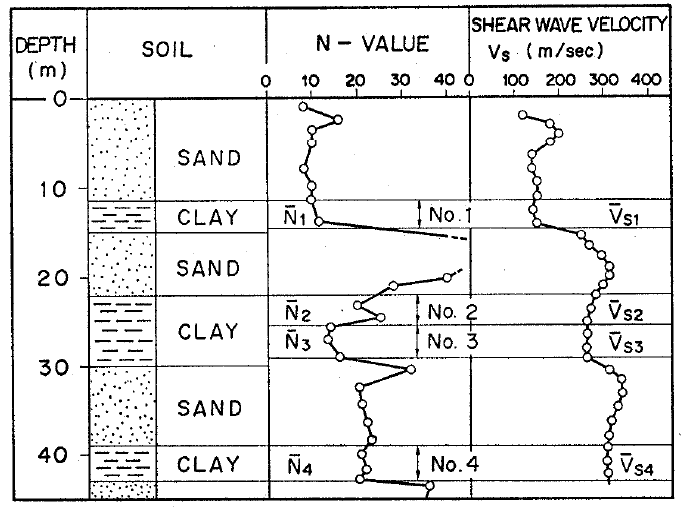
\includegraphics[width=\textwidth]{figures/figure-10.png}
        \caption{An example of data sampling}
        \addtocounter{figure}{-1}
        \vspace{-5pt}
        \renewcommand{\figurename}{图}
        \caption{数据采样示例}
        \renewcommand{\figurename}{Figure}
        \label{figure:10}
    \end{minipage}
    \begin{minipage}[t]{0.46\textwidth}
        \centering
        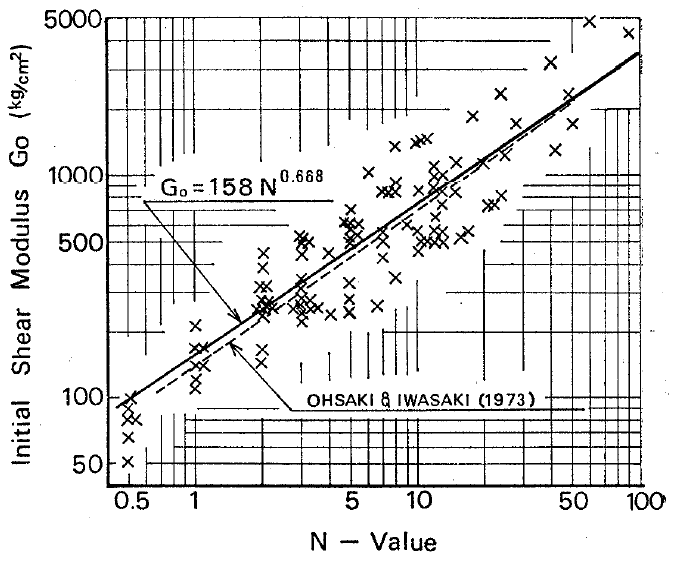
\includegraphics[width=\textwidth]{figures/figure-11.png}
        \caption{Relationship between $G_0$ and N-value}
        \addtocounter{figure}{-1}
        \vspace{-5pt}
        \renewcommand{\figurename}{图}
        \caption{$G_0$和N值之间的关系}
        \renewcommand{\figurename}{Figure}
        \label{figure:11}
    \end{minipage}
\end{figure*}

\Paragraph{Relation between Initial Shear Modulus and N-Value 初始剪切模量与N值之间的关系}

\begin{paracol}{2}
    
    The data on initial shear modulus $G_0$ and N-value thus sampled in conformity with the above criteria of data sampling are plotted on a logarithmic graph as shown in \autoref{figure:11}. \autoref{figure:11} shows that $G_0$ and N-value is in approximate proportion to each other on the logarithmic graph.

    Accordingly, on the assumption that the first order equation should be $G_0=aN^b$ the following empirical formula was obtained by calculating $a$ and $b$ by the least squares method :

    \switchcolumn

    这样按照上述数据采样标准采样的初始剪切模量$G_0$和N值的数据绘制在对数图上,如\cnfigureref{figure:11}所示。图\cnfigureref{figure:11}表明,$G_0$和N值与比例大致成比例。 在对数图中彼此。
       
    因此,假设一阶方程应为$G_0=aN^b$,则通过最小二乘法计算$a$和$b$可获得以下经验公式: 

\end{paracol}

\begin{align}
    G_0=158N^{0.668}(\rm{kg/cm^2})
    \label{equation:9}
\end{align}

\begin{paracol}{2}
    
    \noindent{}where coefficient of correlation $\rho_{xy}=0.88$. 

    \switchcolumn

    \noindent{}其中相关系数$\rho_{xy}=0.88$。

\end{paracol}

\Paragraph{Comparison with Other Investigations 与其他调查研究的比较}

\begin{paracol}{2}
    
    Ohsaki and Iwasaki have evaluated the relation between $G_0$ and N-value by arranging the data obtained from well-shooting tests and standard penetration tests, which were collected by the Evaluation Committee on High-Rise Building Structures, the Building Center of Japan. With classification of soil into cohesive soil and sandy soil with a view to facilitating evaluation of the relation between $G_0$ and N-value, they have shown for cohesive soils that the following empirical formula existed between $G_0$ and N-value:

    \switchcolumn

    \citet{Ohsaki197361}通过安排由日本建筑中心高层建筑结构评估委员会收集的地震测井试验和标准贯入试验获得的数据,评估了$G_0$和N值之间的关系。为了便于评估$G_0$和N值之间的关系,将土壤分为黏性土和砂土,他们表明对于黏性土,在$G_0$和N值之间存在以下经验公式:

\end{paracol}

\begin{align}
    G_0=140N^{0.722}(\rm{kg/cm^2})
    \label{equation:10}
\end{align}

\begin{paracol}{2}
    
    \noindent{}where coefficient of correlation $\rho_{xy}=0.90$. Graphical expression of \autoref{equation:9} and \autoref{equation:10} show that there is quite a similarity between them, as illustrated in Fig. 11.

    \switchcolumn

    \noindent{}其中相关系数$\rho_{xy}=0.90$。 \cnequationref{equation:9}和\cnequationref{equation:10}的图形表明,它们之间有相当的相似性,如\cnfigureref{figure:11}所示。
\end{paracol}